\begin{frame}{Why decompose? Why not Fourier?}
  \begin{block}{Why split the series}
    \begin{itemize}
      \item Raw $Y_t$ mixes noise, diurnal swings, and slow level shifts.
      \item One light model on the mix misses scale-specific structure.
      \item Decompose $\to$ forecast each band $\to$ add back $=$ richer dynamics without a heavy global model.
    \end{itemize}
  \end{block}
  \begin{alertblock}{Why not Fourier}
    \begin{itemize}
      \item Fourier uses \textbf{global} sinusoids over the whole record.
      \item Air quality is \textbf{non-stationary} --- spikes and regime changes are local in time.
      \item Wavelets give a joint \textbf{time--scale} view; MODWT keeps every band length $N$ (no downsampling).
      \item Haar MRA is additive: $Y_t=\sum_k D_{k,t}+S_{K,t}$.
    \end{itemize}
  \end{alertblock}
\end{frame}

\begin{frame}{MODWT: additive components}
  \begin{columns}[T]
    \begin{column}{0.40\textwidth}
      \[
        Y_t = \sum_{k=1}^{K} D_{k,t} + S_{K,t}
      \]
      {\footnotesize
      \begin{itemize}
        \item $D_{k,t}$: detail at scale $\sim 2^{k}$~h.
        \item $S_{K,t}$: smooth after $K$ levels.
        \item Paper: $K\approx\ln N$; we use $K{=}4$--$5$ ($\sim 16$--$32$~h smooth).
        \item $D_1$: high-frequency component;\\
              $D_k$: lower-frequency component;\\
              $S_K$: smooth trend / level.
      \end{itemize}
      }
    \end{column}
    \begin{column}{0.58\textwidth}
      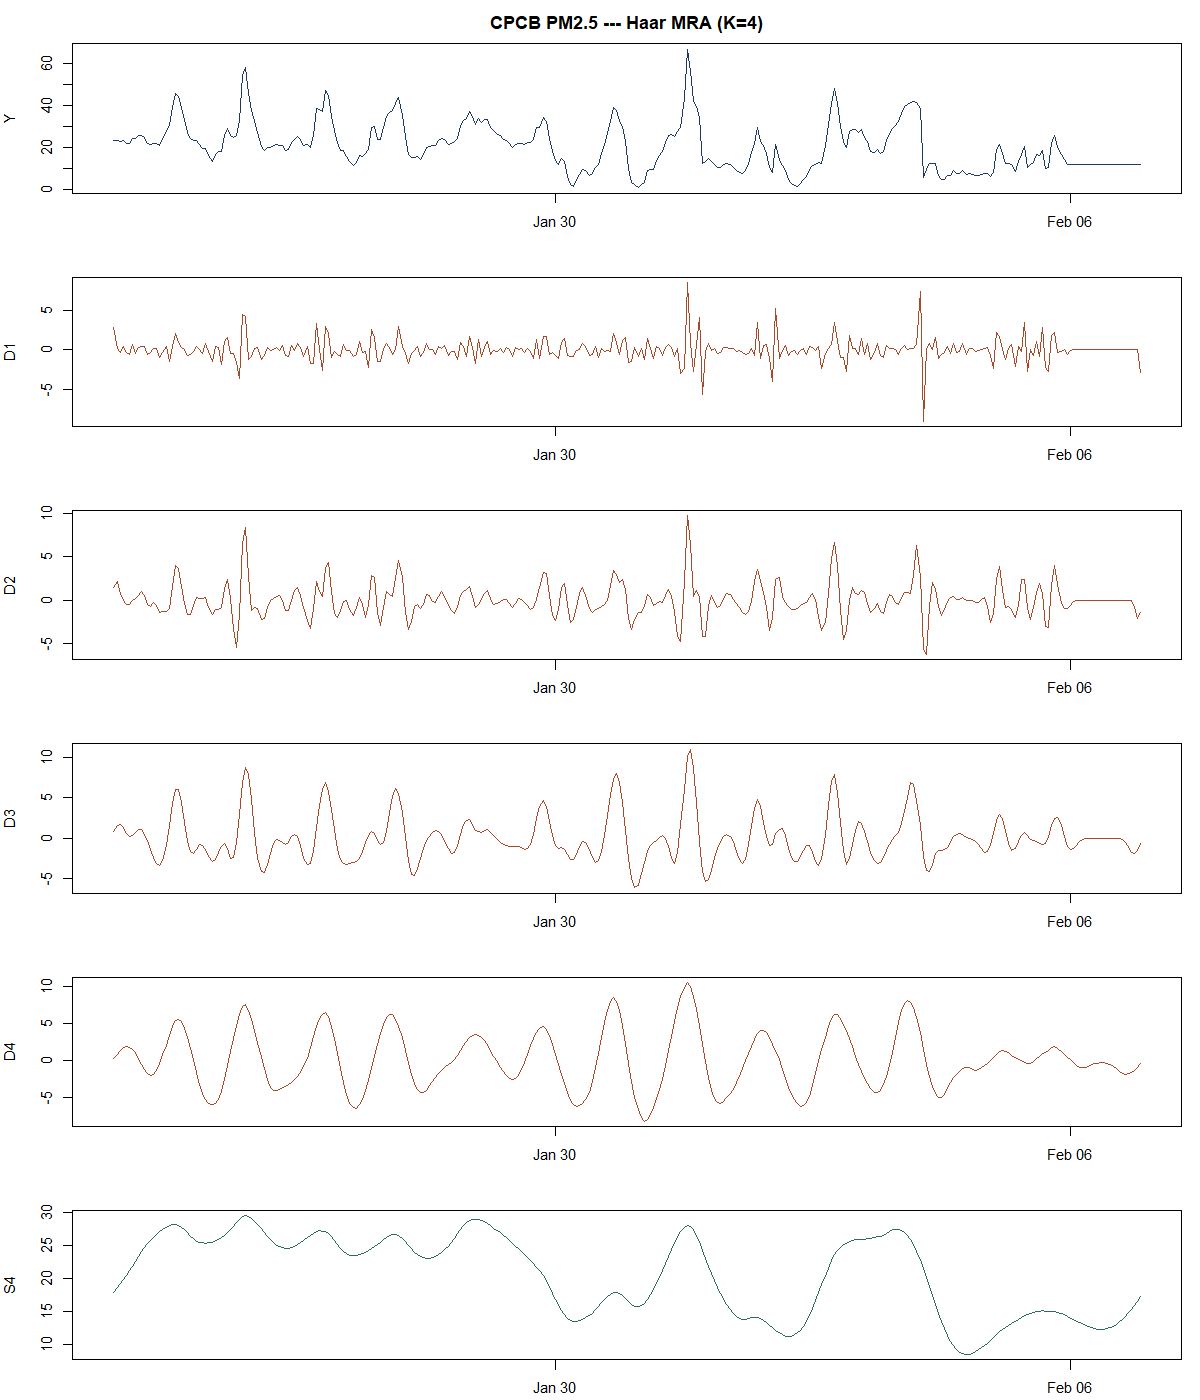
\includegraphics[width=\linewidth,height=0.78\textheight,keepaspectratio]{mra_d1d4_s4_cpcb_pm25.png}
    \end{column}
  \end{columns}
\end{frame}

% Mathematical intuition --- boxed filters like reference slide; compact tree
\begin{frame}{MODWT: mathematical intuition}
  \begin{columns}[T]
    \begin{column}{0.50\textwidth}
      {\scriptsize
      \noindent
      \fcolorbox{gray!55}{gray!12}{\parbox{0.96\linewidth}{%
        \textbf{Wavelet filter:} $p_m\to D$ (details)\\
        $\sum_m p_m=0$ \ (measures change)}}\\[0.3em]
      \fcolorbox{gray!55}{gray!12}{\parbox{0.96\linewidth}{%
        \textbf{Scaling filter:} $q_m\to S$ (smooth)\\
        $\sum_m q_m=1$ \ (measures average)}}\\[0.4em]
      \textbf{Filter condition} (nonzero $n$):\\
      $\sum_m p_m p_{m+2n}=\sum_m q_m q_{m+2n}=0$\\[0.35em]
      \textbf{Recursion at level $j$}\ ($S_{0,t}=Y_t$)\\[0.15em]
      $D_{j,t}=\sum_{m}p_m\,S_{j-1,(t-2^{j-1}m)\bmod N}$\\[0.1em]
      $S_{j,t}=\sum_{m}q_m\,S_{j-1,(t-2^{j-1}m)\bmod N}$\\[0.25em]
      Haar: $q=(\tfrac12,\tfrac12)$,\ $p=(\tfrac12,-\tfrac12)$.\\
      Tap spacing doubles each level.
      }
    \end{column}
    \begin{column}{0.48\textwidth}
      \centering
      \resizebox{0.88\linewidth}{!}{%
      \begin{tikzpicture}[
        font=\scriptsize,
        x=0.72cm, y=0.62cm,
        box/.style={draw, rounded corners=1.5pt, align=center,
                    inner sep=1.2pt, minimum width=0.65cm, minimum height=0.38cm},
        ybox/.style={box, fill=blue!40},
        dbox/.style={box, fill=gray!18},
        sbox/.style={box, fill=gray!18},
        arr/.style={-{Latex}, thick}
      ]
        \node[ybox] (y)  at (0.9, 0) {$Y$};
        \node[dbox] (d1) at (0.0,-1.0) {$D_1$};
        \node[sbox] (s1) at (1.8,-1.0) {$S_1$};
        \node[dbox] (d2) at (0.9,-2.0) {$D_2$};
        \node[sbox] (s2) at (2.7,-2.0) {$S_2$};
        \node[dbox] (d3) at (1.8,-3.0) {$D_3$};
        \node[ybox] (s3) at (3.6,-3.0) {$S_3$};
        \draw[arr] (y)  -- (d1);
        \draw[arr] (y)  -- (s1);
        \draw[arr] (s1) -- (d2);
        \draw[arr] (s1) -- (s2);
        \draw[arr] (s2) -- (d3);
        \draw[arr] (s2) -- (s3);
      \end{tikzpicture}%
      }

      \vspace{0.2em}
      {\scriptsize
      Only the smooth is split again.\\
      $Y=D_1+D_2+D_3+S_3$\\[0.25em]
      \textbf{Inverse (IMODWT):} same filters, reversed\\
      \resizebox{\linewidth}{!}{$
        S_{j-1,t}=\sum_m p_m D_{j,t+2^{j-1}m}
        +\sum_m q_m S_{j,t+2^{j-1}m}
      $}
      }
    \end{column}
  \end{columns}
\end{frame}

\begin{frame}{Filter coefficients}
  \centering
  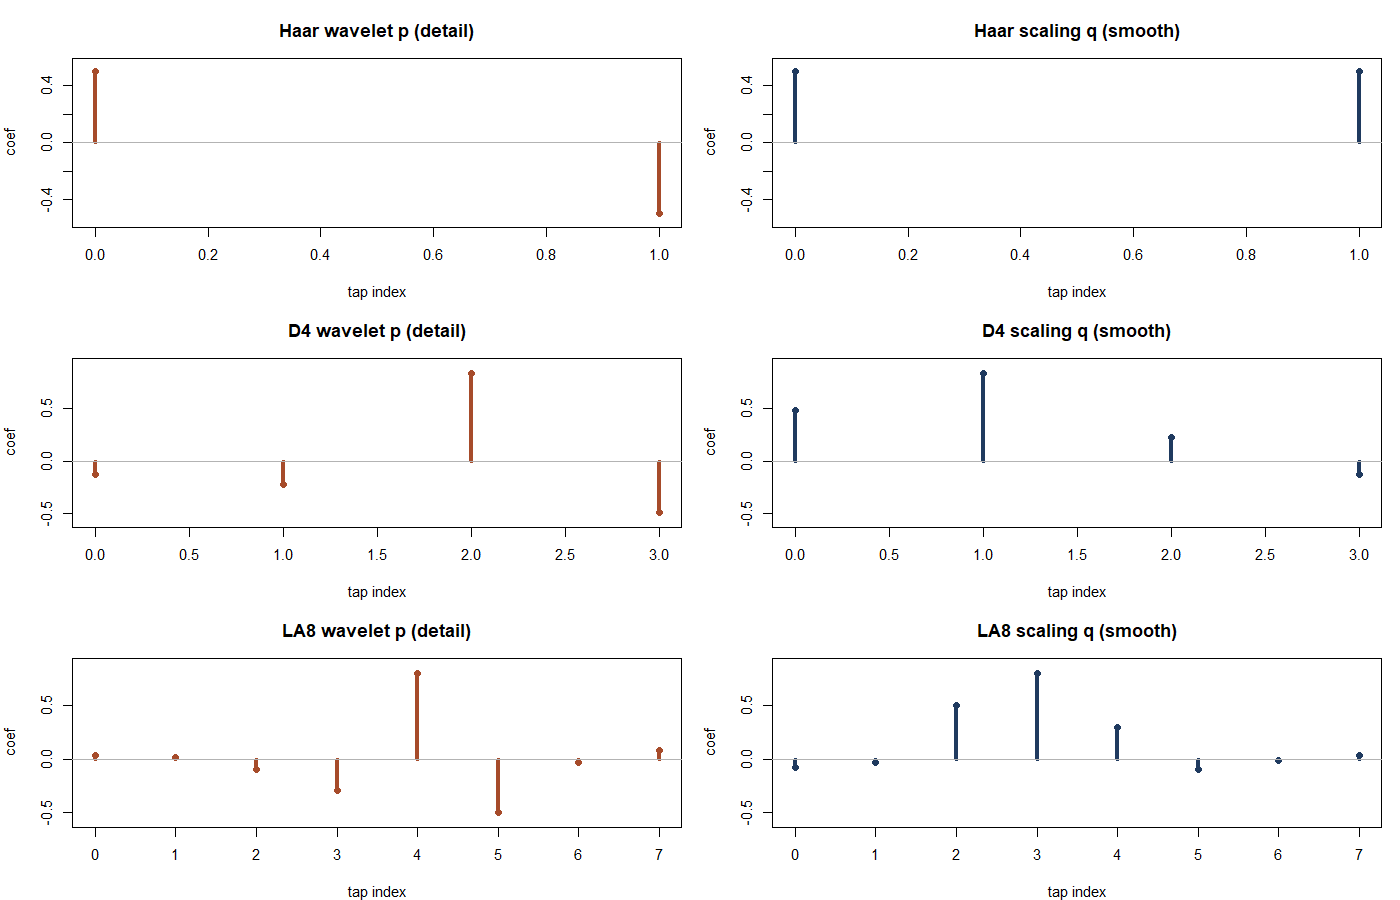
\includegraphics[width=0.95\linewidth,height=0.78\textheight,keepaspectratio]{filter_taps.png}
\end{frame}

\begin{frame}{Haar vs D4 vs LA8 (WaveCatBoost, 1-day MASE)}
  \begin{itemize}\setlength\itemsep{0.2em}
    \item \textbf{Paper default:} Haar ($M{=}2$).
    \item \textbf{We also tried:} D4 ($M{=}4$) and LA8 ($M{=}8$).
    \item Same WaveCatBoost head, same $K$ and lag $p$.
  \end{itemize}
  \vspace{0.4em}
  \centering
  \begin{tabular}{llccc}
    \toprule
    Sensor & Pollutant & Haar & D4 & LA8 \\
    \midrule
    CPCB & NO$_2$    & 0.541 & 0.510 & 0.529 \\
    CPCB & PM$_{2.5}$ & 0.727 & 0.909 & 0.955 \\
    ID1  & NO$_2$    & 1.252 & 1.346 & 1.330 \\
    ID1  & PM$_{2.5}$ & 0.421 & 0.457 & 0.502 \\
    \bottomrule
  \end{tabular}
  \vspace{0.5em}
  \begin{exampleblock}{Takeaway}
    Haar wins on 3 of 4 cells (D4 edges CPCB NO$_2$). Longer filters do not help overall --- Haar stays the default.
  \end{exampleblock}
\end{frame}
